%%%%%%%%%%%%%%%%%%%%%%%%%%%%%%%%%%%%%%%%%%%%%%%%%%%%%%%%%%%%%%%%%%%%%%
% How to use writeLaTeX:
%
% You edit the source code here on the left, and the preview on the
% right shows you the result within a few seconds.
%
% Bookmark this page and share the URL with your co-authors. They can
% edit at the same time!
%
% You can upload figures, bibliographies, custom classes and
% styles using the files menu.
%
% If you're new to LaTeX, the wikibook is a great place to start:
% http://en.wikibooks.org/wiki/LaTeX
%
%%%%%%%%%%%%%%%%%%%%%%%%%%%%%%%%%%%%%%%%%%%%%%%%%%%%%%%%%%%%%%%%%%%%%%
\documentclass{tufte-handout}

%\geometry{showframe}% for debugging purposes -- displays the margins

\usepackage{amsmath}

% Set up the images/graphics package
\usepackage{graphicx}
\setkeys{Gin}{width=\linewidth,totalheight=\textheight,keepaspectratio}
\graphicspath{{graphics/}}

\title{Stata Lab 1: Stata Coding for Reproducible Research}
\author{DIME Analytics \\ dimeanalytics@worldbank.org}
% \date{24 January 2009}  % if the \date{} command is left out, the current date will be used

% The following package makes prettier tables.  We're all about the bling!
\usepackage{booktabs}

% The units package provides nice, non-stacked fractions and better spacing
% for units.
\usepackage{units}

% The fancyvrb package lets us customize the formatting of verbatim
% environments.  We use a slightly smaller font.
\usepackage{upquote}
\usepackage{fancyvrb}
\fvset{fontsize=\normalsize}
\renewcommand{\FancyVerbFormatLine}{\color{violet}}
\DefineShortVerb{\|}

% Small sections of multiple columns
\usepackage{multicol}

% Provides paragraphs of dummy text
\usepackage{lipsum}

% These commands are used to pretty-print LaTeX commands
\newcommand{\doccmd}[1]{\texttt{\textbackslash#1}}% command name -- adds backslash automatically
\newcommand{\docopt}[1]{\ensuremath{\langle}\textrm{\textit{#1}}\ensuremath{\rangle}}% optional command argument
\newcommand{\docarg}[1]{\textrm{\textit{#1}}}% (required) command argument
\newenvironment{docspec}{\begin{quote}\noindent}{\end{quote}}% command specification environment
\newcommand{\docenv}[1]{\textsf{#1}}% environment name
\newcommand{\docpkg}[1]{\texttt{#1}}% package name
\newcommand{\doccls}[1]{\texttt{#1}}% document class name
\newcommand{\docclsopt}[1]{\texttt{#1}}% document class option name

\begin{document}

\maketitle% this prints the handout title, author, and date

\begin{marginfigure}%
  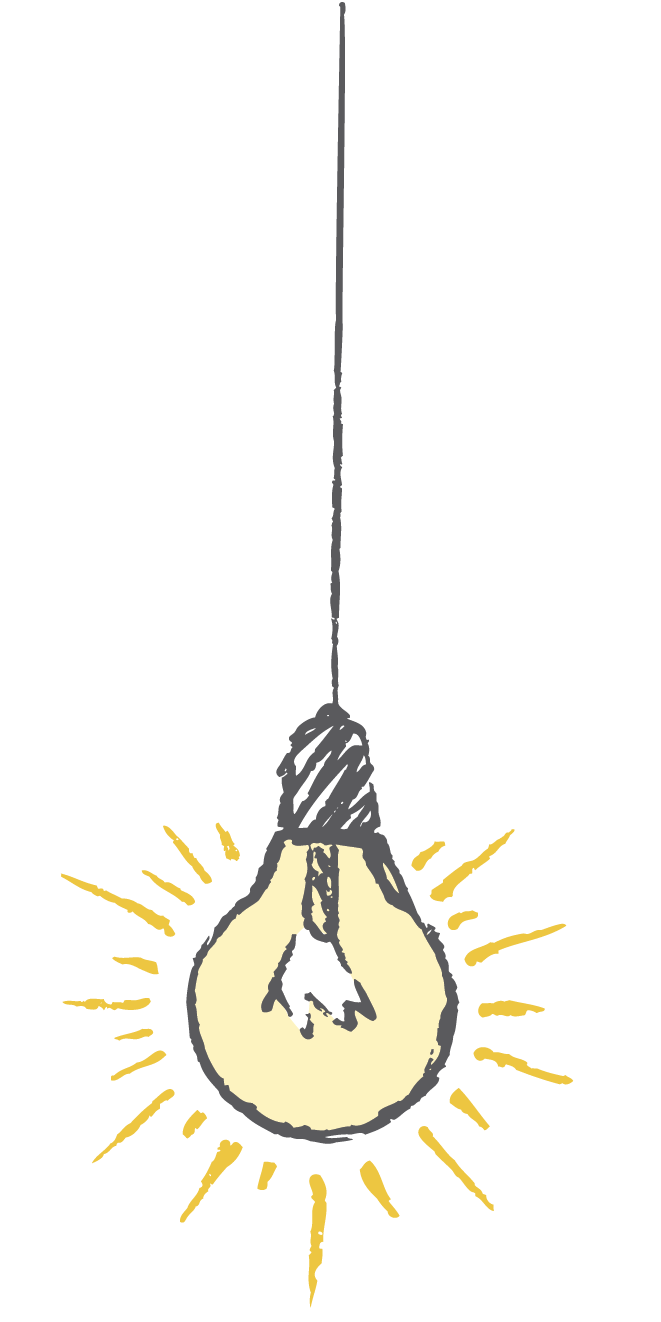
\includegraphics[width=\linewidth]{light.png}
\end{marginfigure}

\begin{abstract}
In this exercise you will be introduced to the DIME template for master do-files,
and learn best practices to use when coding in a team.

\bigskip\noindent \textbf{Exercise Objectives}:
\begin{enumerate}
  \item Set up folder structure for a project
  \item Set up a dynamic master do-file
  \item Practice writing replicable code
\end{enumerate}
\end{abstract}

%\printclassoptions
\section{Part 1: Setting up your working directory}

Create a top-level folder for |/Field Coordinator Training/|.
This folder will be used during the training sessions
and you will save your lab materials in it.
Make sure you know the \textbf{absolute filepath} to this location:
you will need to use it occasionally.
That filepath will be something like:
\begin{Verbatim}
  /users/bbdaniels/Dropbox/MSIE 2019/
\end{Verbatim}
on a Mac; or
\begin{Verbatim}
  C:/users/bbdaniels/Dropbox/MSIE 2019/
\end{Verbatim}
on a PC. Make sure you are able to copy-and-paste that path.
Also, make sure you copy the path using \textbf{forward slashes} (|/|),
like you are writing a web URL. Think of this path the same way.
Do this always. You will see that we use that style everywhere.
The reason is that the other style will not run on non-PC machines.

Then, open Stata and install the |ietoolkit|\sidenote{\url{https://dimewiki.worldbank.org/wiki/ietoolkit}} package:
\begin{Verbatim}
  ssc install ietoolkit, replace
\end{Verbatim}
This will install the |ietoolkit| package if you don’t have it
and update it you if already have it.
|ietoolkit| is a set of standardized commands for Stata
written by DIME Analytics.
These command make basic Stata tasks much easier,
and ensure that all of our projects and people do them the same way.
Open a \textbf{do-file editor}.
You don't have to use the built-in Stata editor
and we recommend that you use something like Atom or Sublime.
Don't switch now if you haven't already,
but this can make your life a lot easier.

In the new do-file editor, we will write a simple setup dofile
to create a new project for us using the DIME Analytics template.
Save this file as |master.do|, directly in the top-level directory
that you created. Therefore, its filepath will be something like:
\begin{Verbatim}
  /users/bbdaniels/Dropbox/MSIE 2019/master.do
\end{Verbatim}
At the very beginning of this file, write its purpose in a comment.
You can use |//| or |*| for comment lines; either will do. (I prefer |//|.)
The purpose of this file is to "Set up the folder for Stata Track 2."
At the beginninf of such a master file, we will want to make sure
that we have standardized core Stata settings.
For this, |ietoolkit| includes a command called |ieboilstart|.\sidenote{\url{https://dimewiki.worldbank.org/wiki/ieboilstart}}
It is written as follows:
\begin{Verbatim}
  ieboilstart, v(12.1)
  `r(version)'
\end{Verbatim}
Two lines are required because Stata does not allow |ieboilstart|
to change the Stata \textbf{version} – you have to do this manually.
Check that it is now available in |return| by typing |return list|.
Setting the version of Stata is very important to make sure
your code will work across other machines.

Then, ask Stata to remember where your top-level directory is
using a \textbf{global macro}. A global macro is a name
stored in Stata's memory that you can use in place of a long one.
Global macros do not do anything more than that:
they are placeholders, and their contents get substituted in for them
when you run the Stata code. Write:
\begin{Verbatim}
  global directory "/users/bbdaniels/Dropbox/MSIE 2019/"
\end{Verbatim}
replacing the filepath with yours.
Run this code, then type
\begin{Verbatim}
  di "${directory}"
\end{Verbatim}
in Stata. It will show you the contents of the macro named |directory|.
Those contents -- which in reality are just a bunch of letters --
can be used as shorthand for the location of your work.
This macro and its contents has no other special meaning; use anything you like.

Next, use |iefolder|\sidenote{\url{https://dimewiki.worldbank.org/wiki/iefolder}}
to create a new |/DataWork/| folder in the |/Field Coordinator Training/| folder.
Type |help iefolder| to check how this is done.
In general, we will not explain Stata commands extensively;
you should take some time to become familiar with how to read helpfiles.
In particular, you will need to know how to figure out Stata \textbf{syntax}
from the layout of the helpfile.
You should have written:
\begin{Verbatim}
  iefolder new project, project("${directory}")
\end{Verbatim}

Take a look at the contents of the new |/DataWork/| folder.
In particular, open |Project_MasterDofile.do|.
This file is created automatically by |iefolder|,
and because the structure of the folder is standard,
It can automatically sets up a further series of global macros
with the file path to this folder and its subfolders.

Now use |iefolder| to create a new ``subfolder''.
Call it |/Lab1/|. This is the folder you’ll work from during this session.
(In the future, you are more likely to use new ``round'' folders,
as they come with additional structure,
but we will keep it simple for now.)
You should have written:
\begin{Verbatim}
  iefolder new subfolder Lab1, project("${directory}")
\end{Verbatim}
Check that |Project_MasterDofile.do| now defines globals
with file paths to the new folder.
Explore the contents of your |/Lab1/| folder.
Finally, use |iefolder| once more to create a new subfolder,
and use |iegitaddmd|\sidenote{\url{https://dimewiki.worldbank.org/wiki/iegitaddmd}}
to make sure all these folders have |README.md| files.
These files are important for making sure folders can be documented and synced.
Call this one |/Lab3/|. You will use this folder in the next lab session.
We suggest you create one such folder for each lab session you’ll have this week
and adapt it to the lab’s needs. If you like, you can do that now.
If you like, you can use a |forvalues| loop for all the labs.
When this dofile is done, it might look like:

\begin{figure*}
{\setstretch{0.7}
\VerbatimInput[frame=lines,numbers=left,label=master.do]{../master.do}}
\end{figure*}

\section{Part 2: Apply techniques from this lesson to demo code}

\subsection{Cleaning dofile}

In this part you will be use the do-files in the Field Coordinator Training folder
and improve them for readability.
Before you start the exercises, make sure you run the new |Project_MasterDofile.do|.
This will store globals with filepaths you will use to load your data.

You will find a data file, |/data/endline_data_raw_nodup.dta|
in the public Field Coordinator Training folder.
Save this dataset to |/DataWork/Lab1/|.
This data has already been de-identified.
Raw data is data that still has personal information.
Final data is data that has been cleaned
and has the constructed or derived variables that will be used for analysis.

You will also find a |.do| file, |/dofiles/Lab1-cleaning.do|
in the public Field Coordinator Training folder.
Save this dofile as |/DataWork/Lab1/cleaning.do| and open it in Stata.
Edit this file.
Use the global |Lab1| to load the |endline_data_raw_nodup.dta| data set
by adding a line in the beginning of the dofile you just opened.
You should write something like:
\marginnote{Reminder: You should always use quotation marks around filepaths,
you should always use \{ \} around globals, and you should always use “/” in filepaths.}
\begin{Verbatim}
  use "${Lab1}/endline_data_raw_nodup.dta" , clear
\end{Verbatim}
|Lab1| is a global macro defined in |Project_MasterDofile.do|
specifying the file path to the |/Lab1/| folder.
It was created automatically by |iefolder|.

See what you can do to improve this do-file
based on the techniques in the presentation.
The .do file corresponds to the data set |endline_data_raw_nodup.dta|.
You will need to open both the do-file and |browse| and |describe|
the data set in order to understand what the do-file is supposed to do.
Can you make it clearer which dataset this depends on?
Would someone else be able to understand what the code is doing?
Would someone else be able to run this dofile?
Could you improve the readability?
Are there ways to improve the coding through macros?

The techniques taught in this lab are not only to make the code more legible.
Open the file |Lab1-cleaning.do| again.
We intentionally put in a bug. Can you find it?
It is hard to find even when you know it is there.
Simplifying code helps the reader,
and is one of the best methods to protect your work from coding bugs.
When you are done, the file might look as shown below.

\begin{figure*}[h]
{\setstretch{0.7}
\VerbatimInput[frame=lines,numbers=left,label=cleaning.do]{../DataWork/Lab1/cleaning.do}}
\end{figure*}

\subsection{Analysis dofile}

Your dofile should now create a |.dta| file,
|/DataWork/Lab1/endline_data_final.dta|.
If not, get this file from |/Materials/endline_data_final.dta|
in the public Field Coordinator Training folder.
You will find another dofile, |Lab1-analysis.do|,
in the public Field Coordinator Training folder.
Save this dofile as |/DataWork/Lab1/analysis.do| and open it.

Use the global |Lab1| that specifies the file path
to the Lab 2 folder to load this data set
by adding a line in the beginning of the do-file you just opened.
|Lab1| is a global defined in |Lab1_MasterDofile.do|
specifying the file path to the folder.
It is created automatically by |iefolder|/
See what you can do to improve the dofile
based on the techniques in the presentation.
The dofile corresponds to the dataset you just opened,
|endline_data_final.dta|.
You will need to open both the dofile and the data set
in order to understand what the dofile is supposed to do.
When you are done, it might look like the one below.

\begin{figure*}[h]
{\setstretch{0.7}
\VerbatimInput[frame=lines,numbers=left,label=analysis.do]{../DataWork/Lab1/analysis.do}}
\end{figure*}

\section{Part 3: Work with a master dofile}

Open |Project_MasterDofile.do| and make changes to it
in ``PART 3: - RUN DOFILES CALLED BY THIS MASTER DOFILE''
so that you can run both the dofiles you worked on during this session
by running only the master dofile.
Then, run |Lab1_MasterDofile.do| and verify
that both the cleaning and analysis dofiles were executed.

It might look like:

\begin{Verbatim}[frame=leftline,numbers=left]
*iefolder*3*RunDofiles**********************************************************
*iefolder will not work properly if the line above is edited

   * ******************************************************************** *
   *
   *       PART 3: - RUN DOFILES CALLED BY THIS MASTER DOFILE
   *
   *           - When survey rounds are added, this section will
   *            link to the master dofile for that round.
   *           - The default is that these dofiles are set to not
   *            run. It is rare that all round-specfic master dofiles
   *            are called at the same time; the round specific master
   *            dofiles are almost always called individually. The
   *            exception is when reviewing or replicating a full project.
   *
   * ******************************************************************** *

   // Lab 2: Stata Coding for Reproducible Research
     if (1) do "${Lab1}/cleaning.do"
     if (1) do "${Lab1}/analysis.do"
\end{Verbatim}

Thanks to the template creators.\cite{tuftelatex}

\bibliography{sample-handout}
\bibliographystyle{plainnat}

\end{document}
